\documentclass[a4paper]{jsarticle}
\setlength{\baselineskip}{16pt}
\setlength{\parskip}{6mm}

% Packages
\usepackage[top = 20truemm, bottom = 20truemm, left = 30truemm, right = 30truemm]{geometry}
\usepackage{amsmath} % For mathematical equations
\usepackage{cite} % For citations
\usepackage{hyperref} % For hyperlinks
\usepackage[dvipdfmx]{graphicx}
\usepackage{here} % For figure placement

% Title and author
\title{中級ミクロデータサイエンス期末課題\\Problem Set 2}
\author{横浜国立大学経済学部3年\\学籍番号 2125178\\廣江友哉}

\begin{document}

\maketitle

ソースコードは、\url{https://github.com/tomoyahiroe/replication-project} にある。リポジトリページ下部の README.md ファイルを参照いただきたい。各Problem Set についての説明を記述している。

\section*{(a)記述統計}

\subsection*{a-1, 問題背景などを知る上で役に立つ記述統計を作成し、内容について議論しなさい}
\begin{figure}[h]
  \centering
  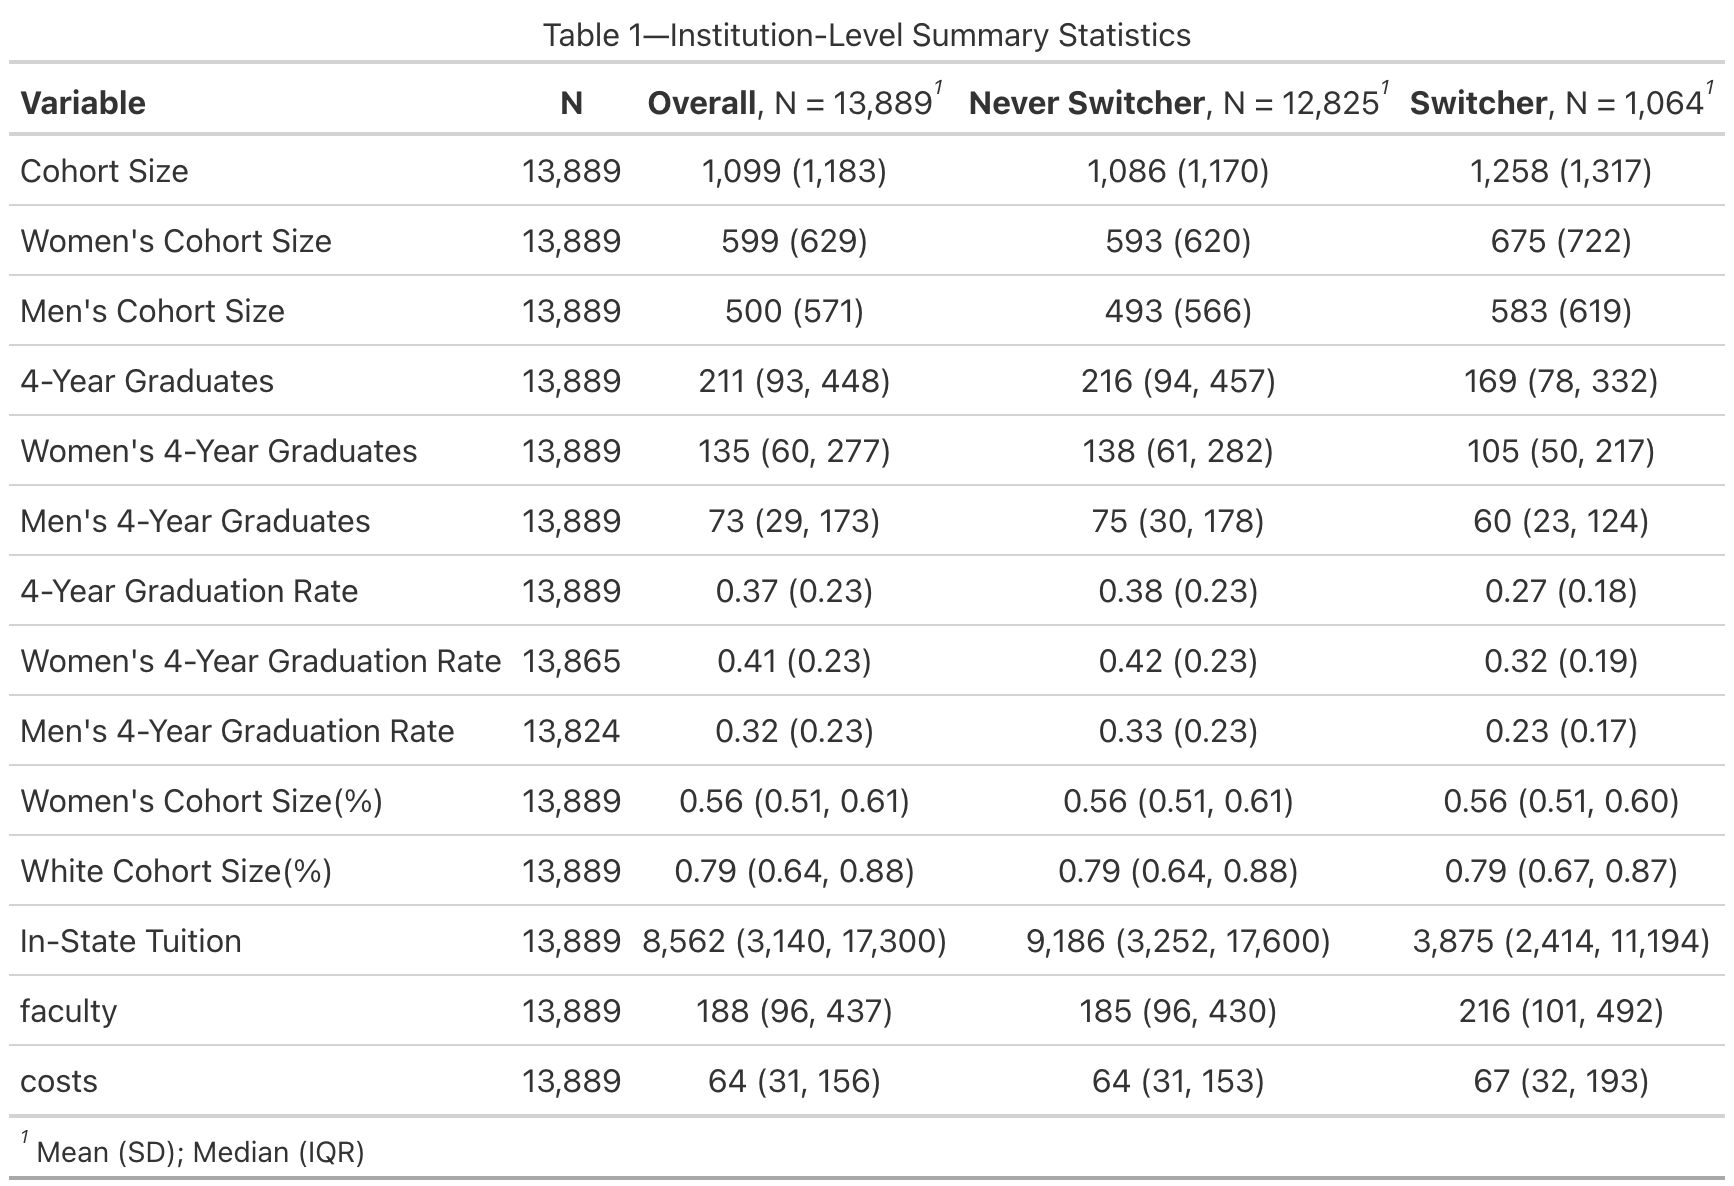
\includegraphics[width = \hsize]{\$HOME/code_box/learn/R/replication-project/src/analyze/output/table/table_1.png}

\end{figure}

クオーター制からセメスター制への移行を1991年から2005年までの間に行った大学は調査対象の大学731校中56校だった。これは元論文の "Switcher"\footnote{Switcher ... クォーター制からセメスター制に変更があった大学} 76校と比較してだいぶ少ない数となっているため、Rで書いたコードの中に誤りが含まれる、もしくは、そもそもの計算方法に誤りがある可能性がある。女性の4年卒業率は男性の四年卒業率と比較して高い傾向にあり、これは "Switcher" "Never Switcher" に関わらず共通している。一方で、卒業率や卒業者数を確認すると、4年卒業率は "Switcher" で 27\% ± 18\%、"Never Switcher" で 38\% ± 23\% となっている。男性についても4年卒業率を確認すると、"Switcher" で 23\% ± 17\%、"Never Switcher" で 33\% ± 23\% となっており、女性は、"Switcher" で 32\% ± 19\%、"Never Switcher" で 42\% ± 23\% となっている。従ってセメスター制への移行を決断する大学は、4年卒業率が低い傾向にあると言える。

\subsection*{a-2, 4年卒業率の平均推移を計算し、図で示しなさい}

各年ごとにすべての大学の4年卒業率の平均を計算し、図で示すと以下のようになる。

\begin{figure}[H]
  \centering
  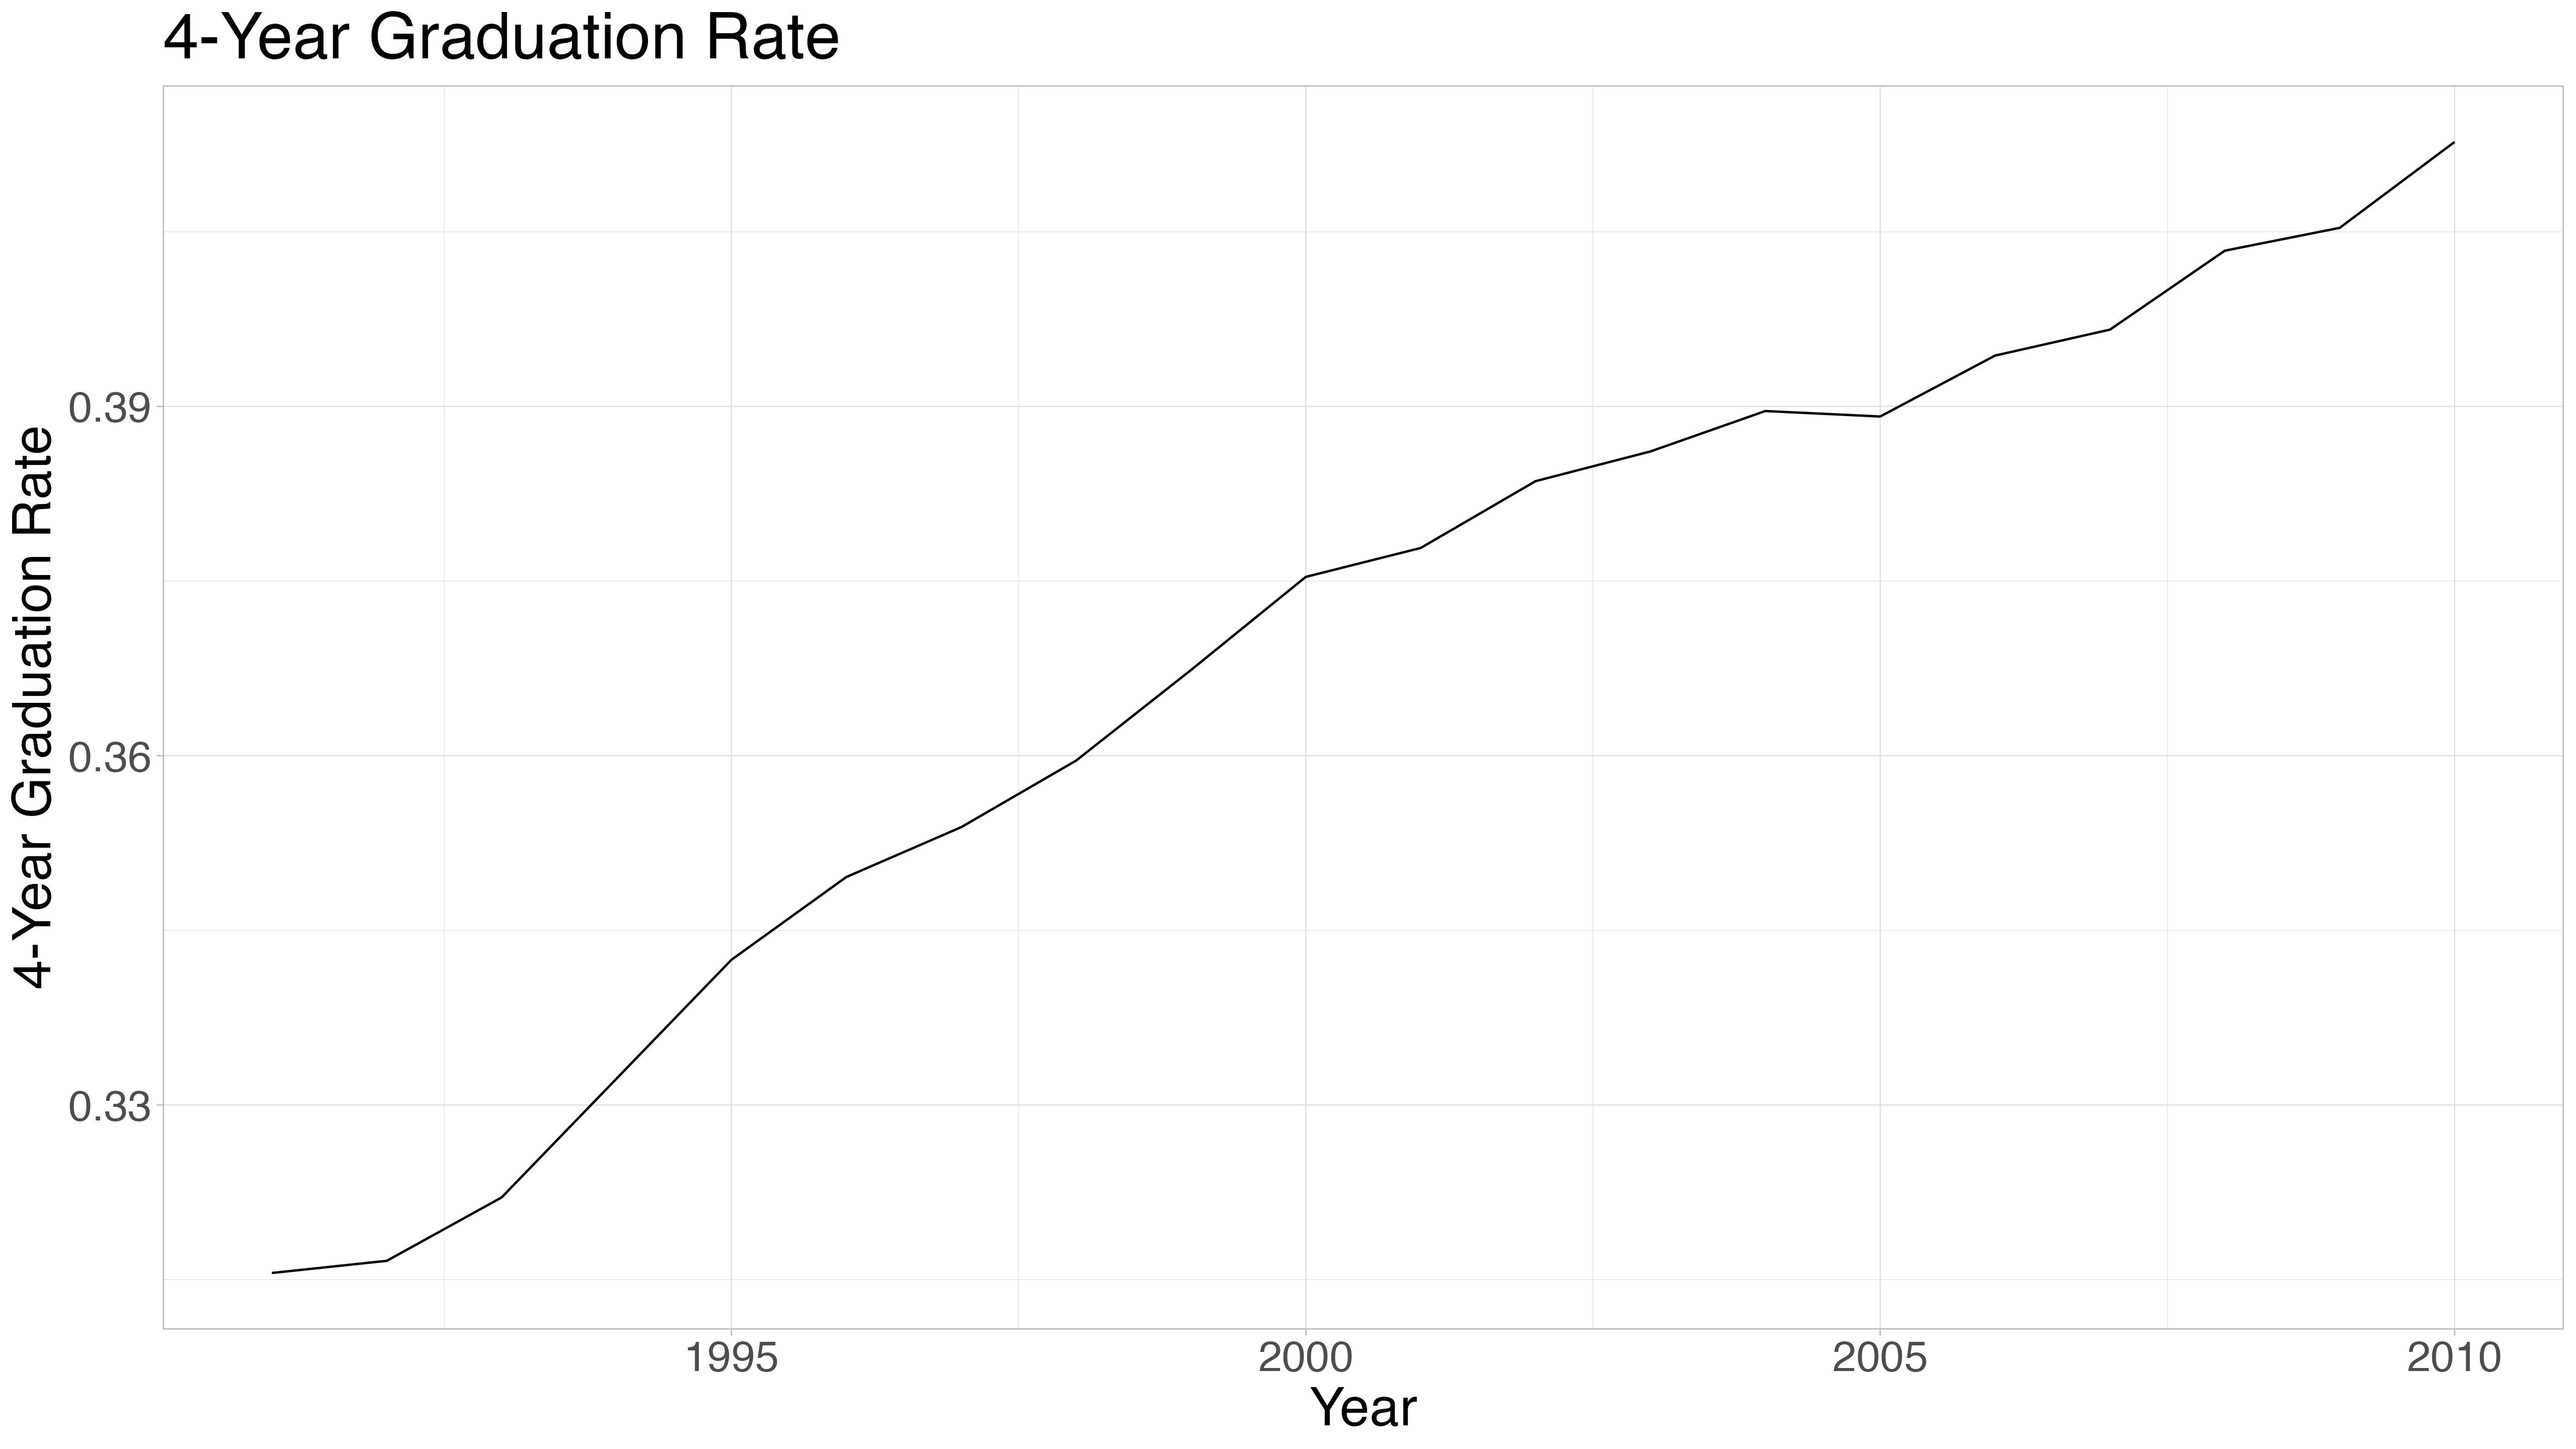
\includegraphics[width = \hsize]{\$HOME/code_box/learn/R/replication-project/src/analyze/output/figure/gradrate_trend.png}

\end{figure}

\subsection*{a-3, semester導入率を計算し、図で示しなさい}

\begin{figure}[H]
  \centering
  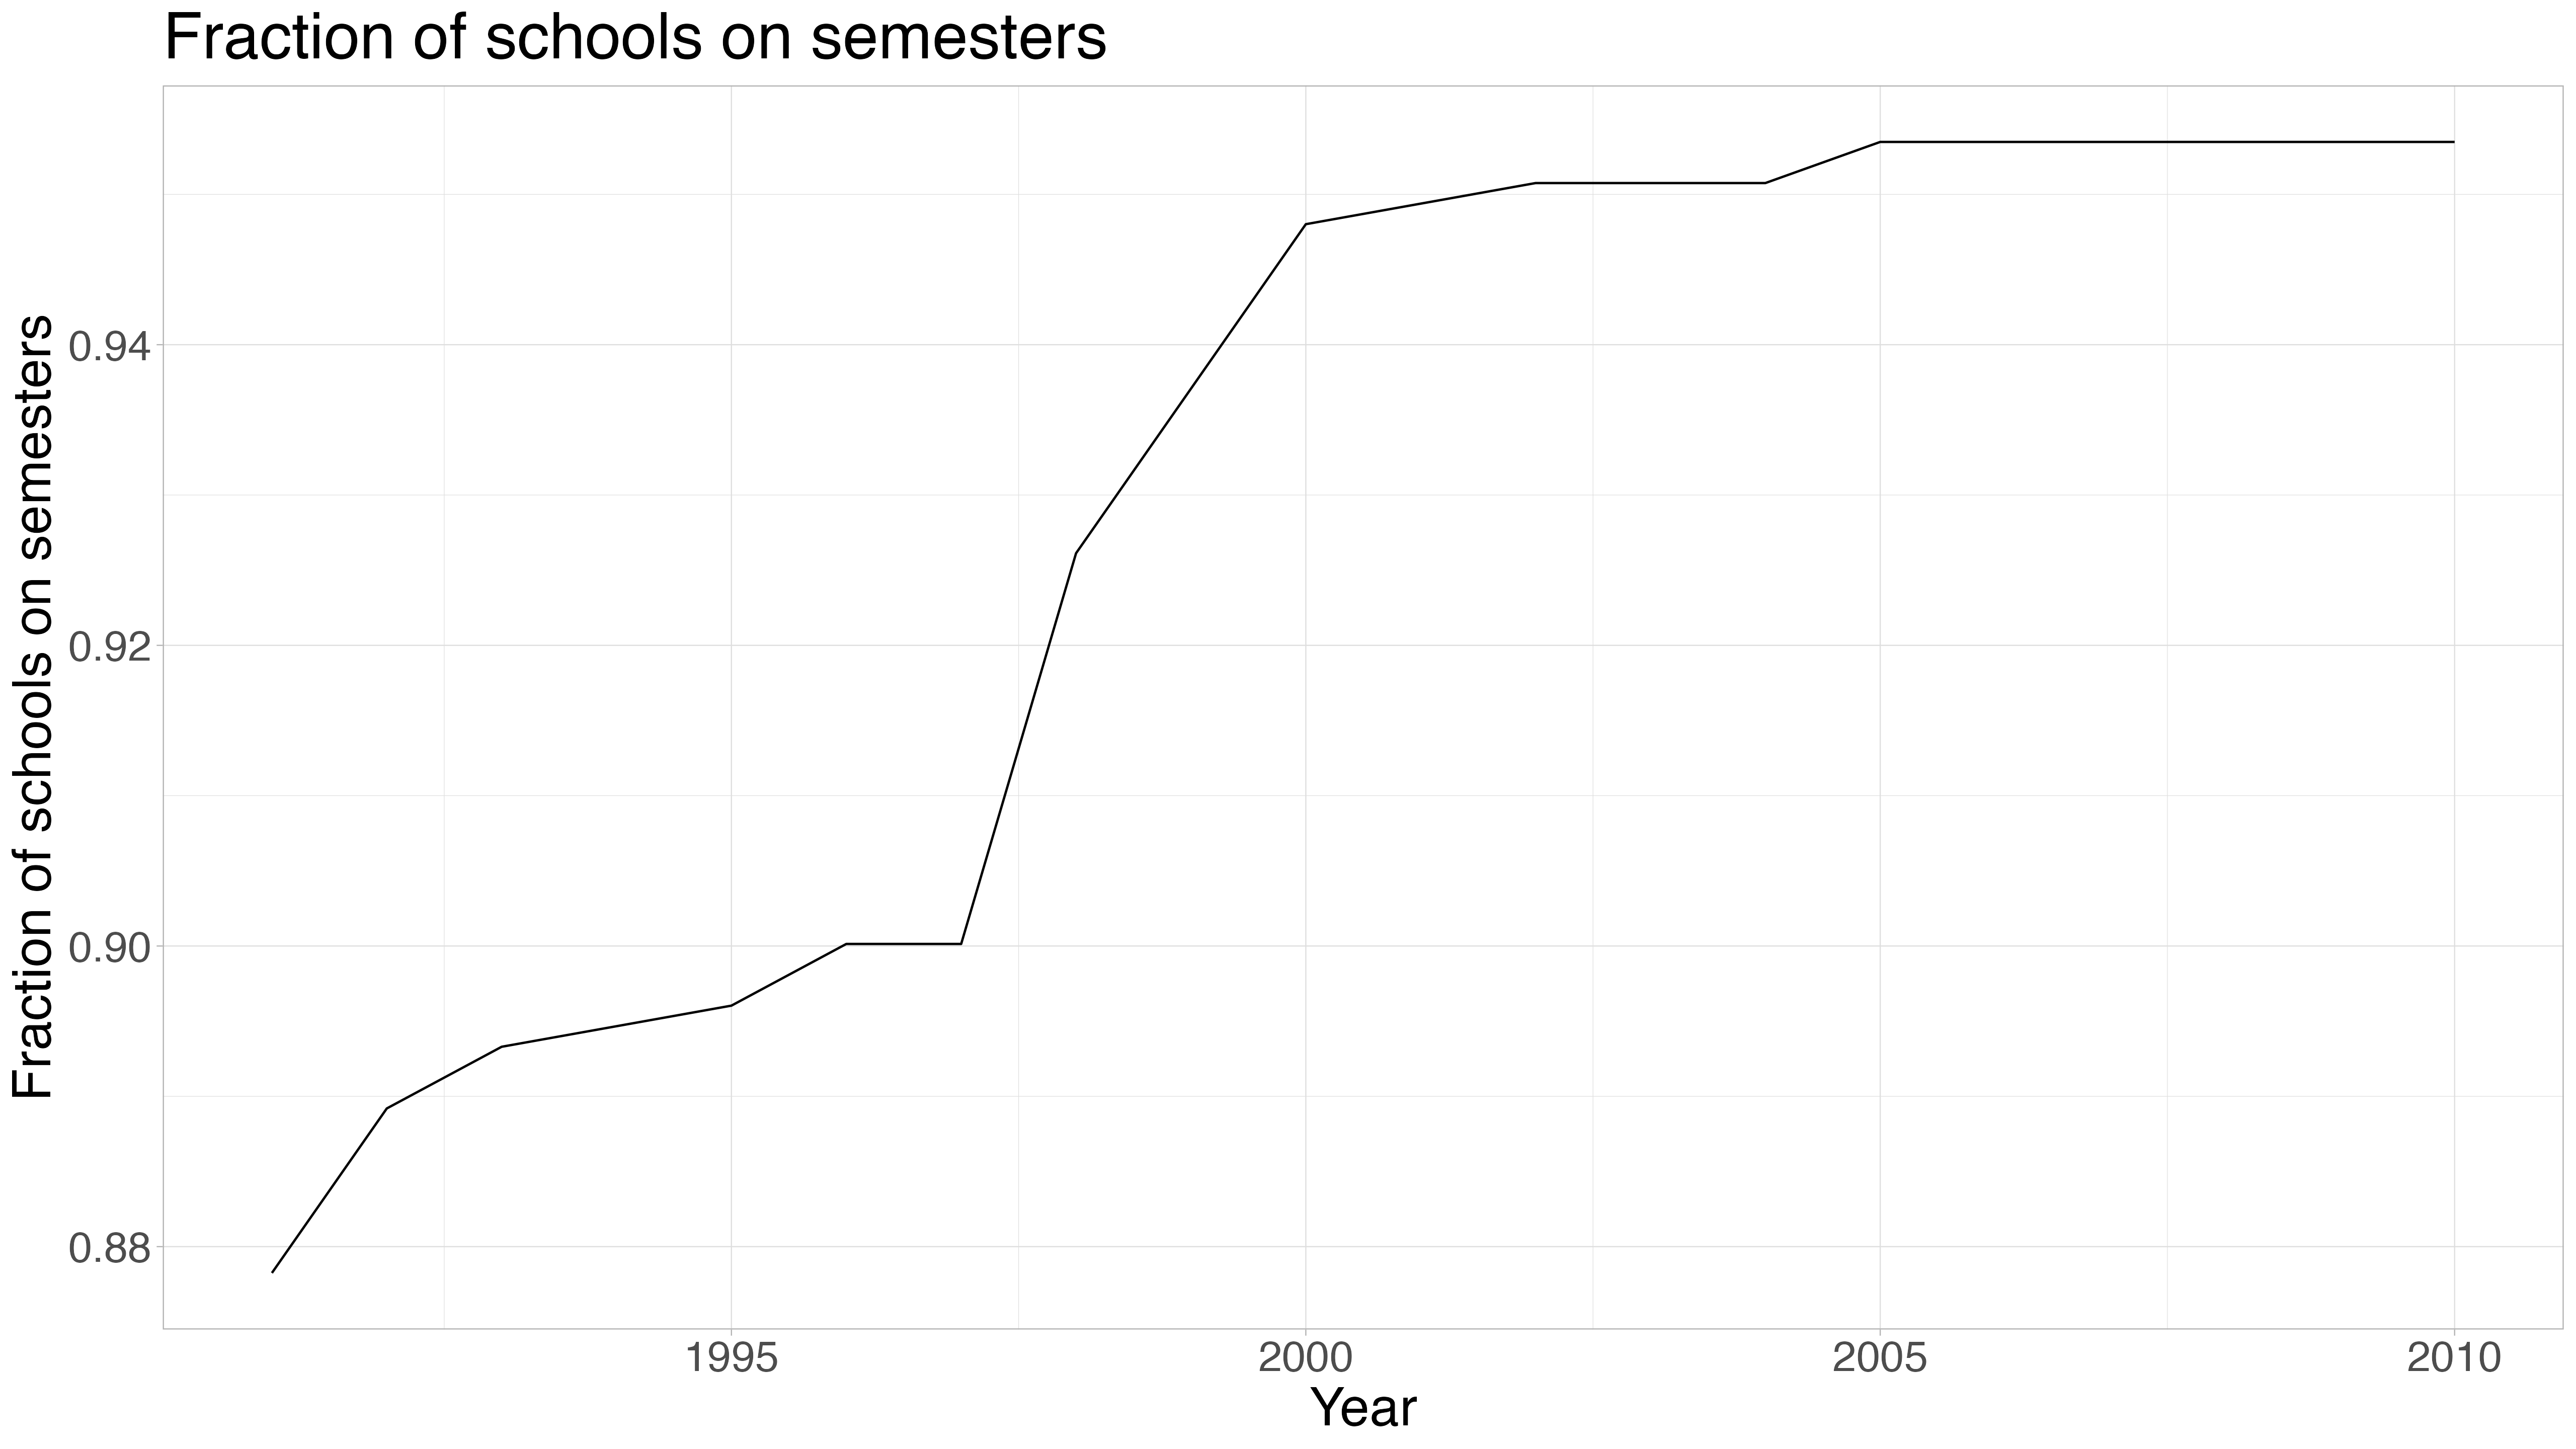
\includegraphics[width = \hsize]{\$HOME/code_box/learn/R/replication-project/src/analyze/output/figure/semester_trend.png}

\end{figure}

\subsection*{a-4, 変数に処理を加えた上で、以下の散布図を作成しなさい。また、重要だと考える結果について議論しなさい}

\begin{figure}[H]
  \centering
  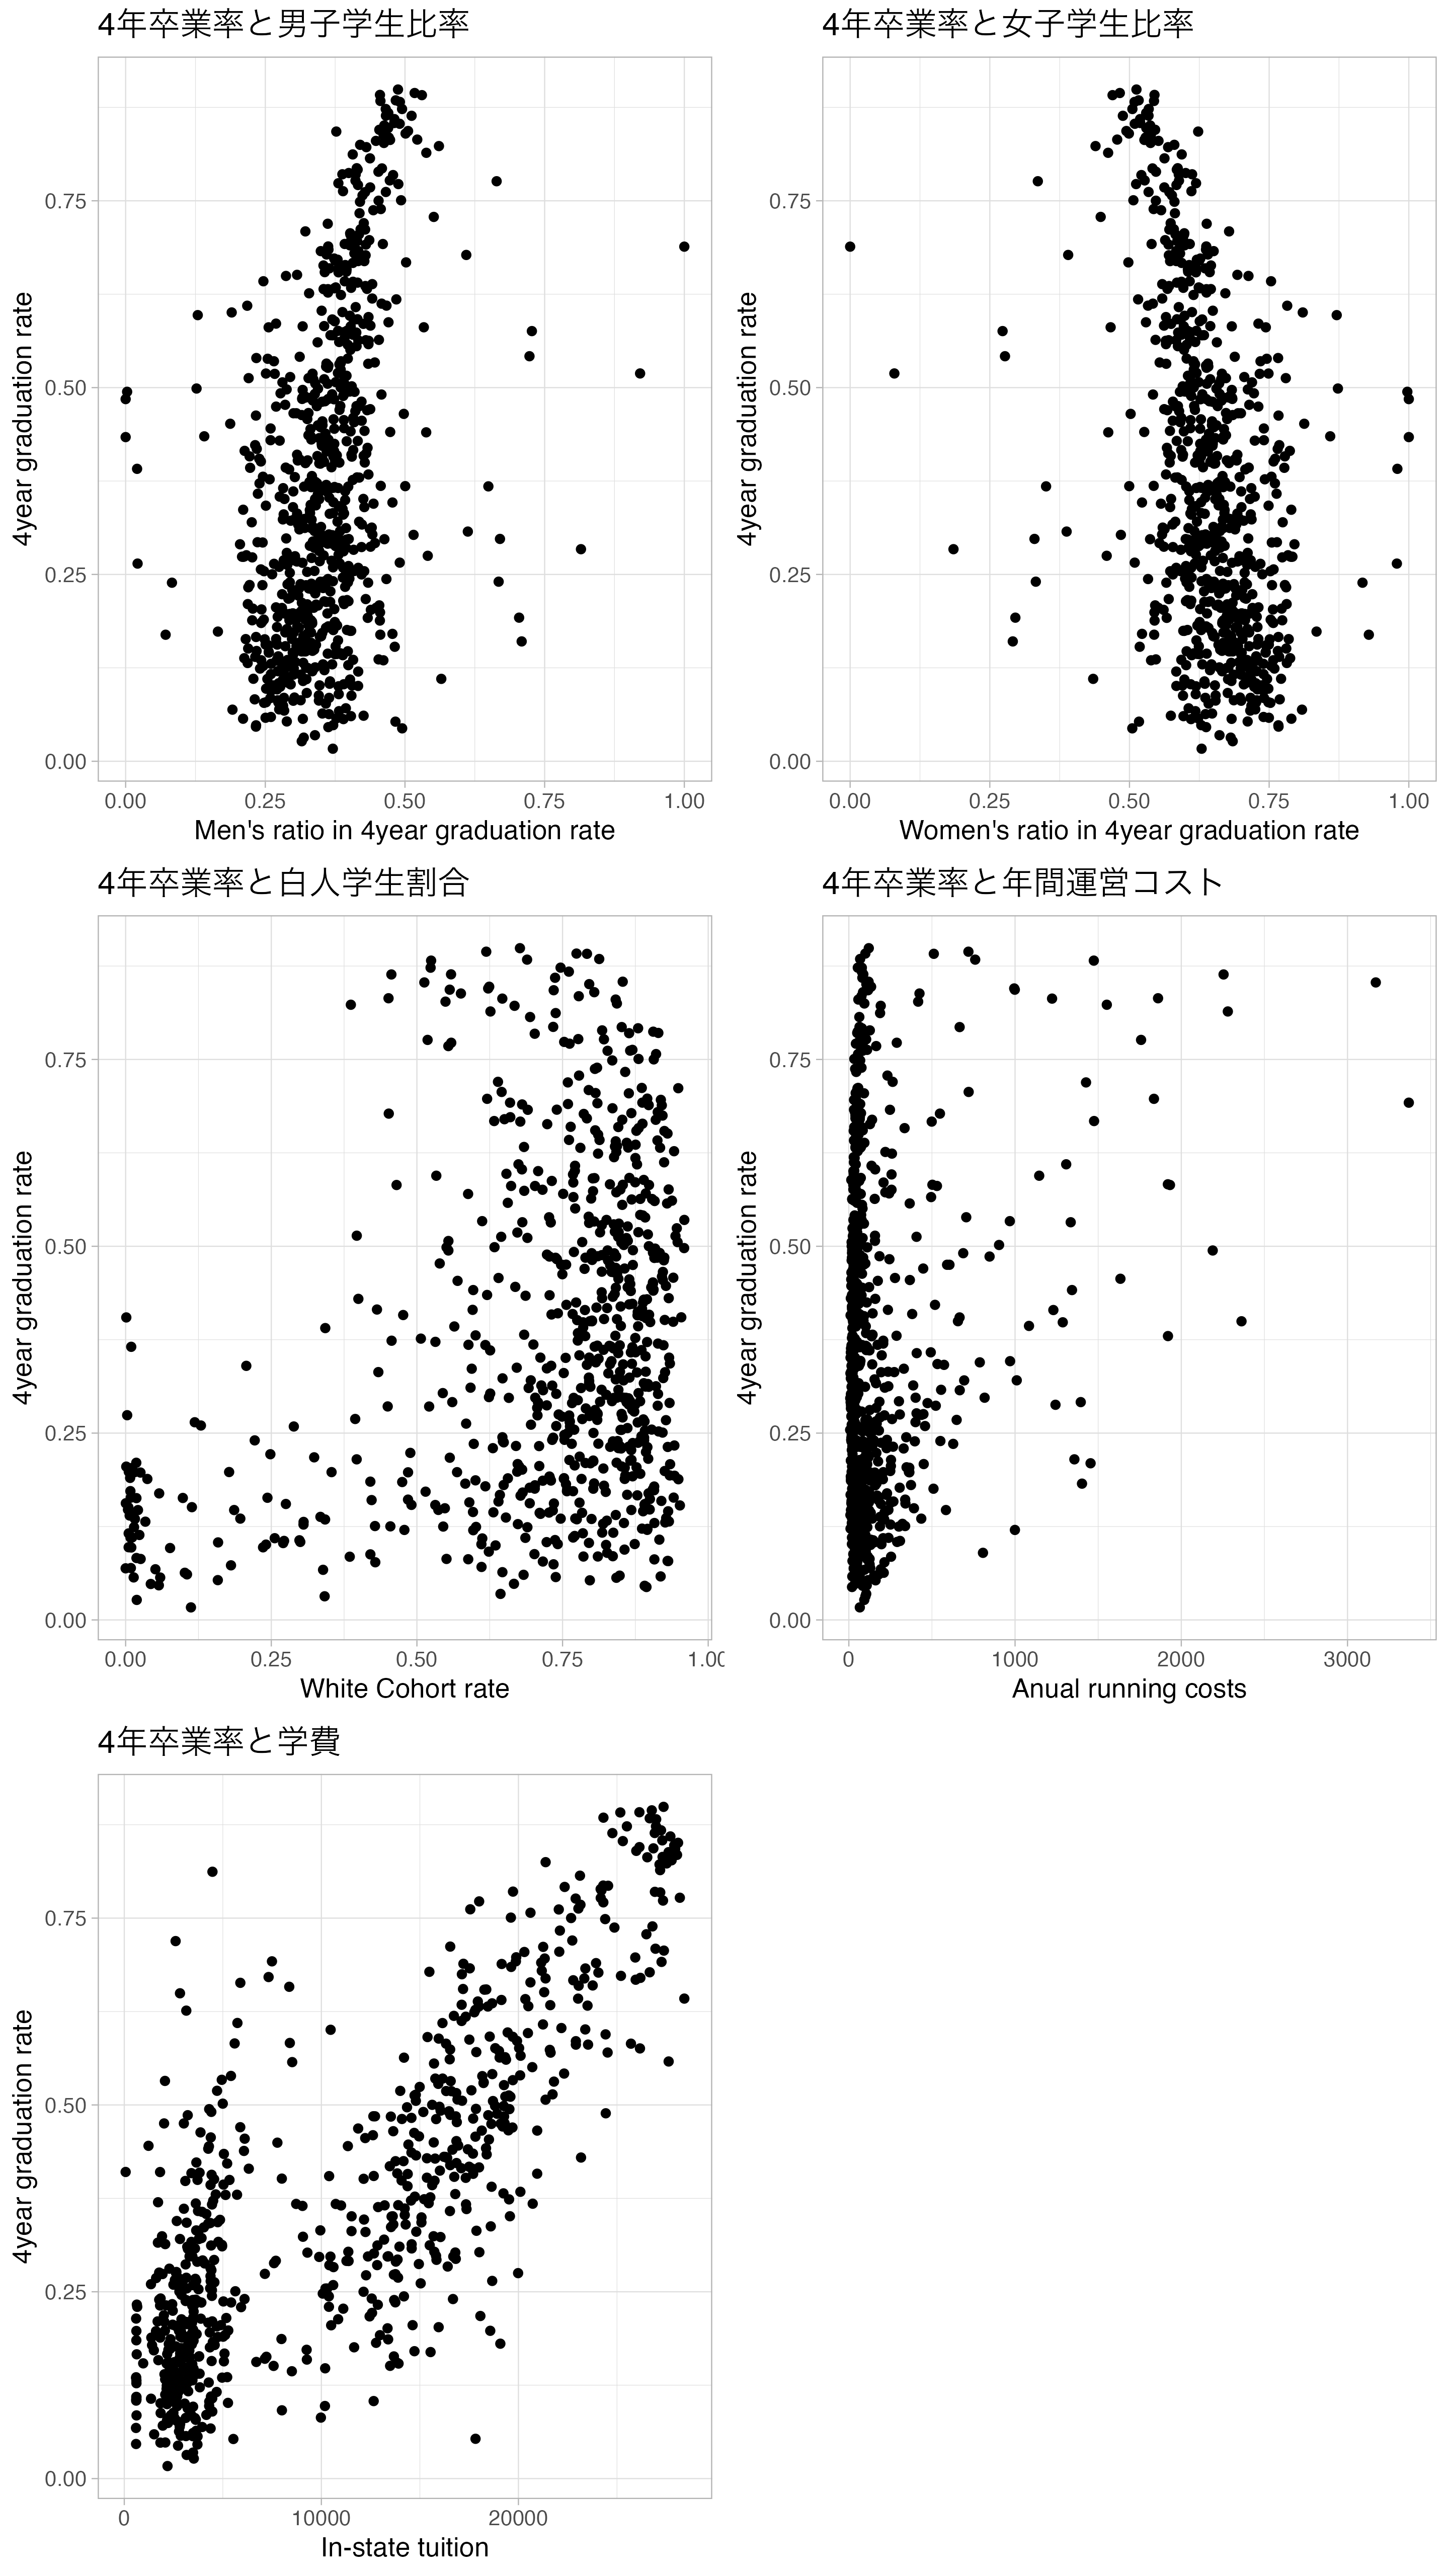
\includegraphics[width = 0.9\hsize]{\$HOME/code_box/learn/R/replication-project/src/analyze/output/figure/scatter_plots.png}

\end{figure}


五つの散布図から読み取れるとこで特徴的なのは、学費と4年卒業率に強い相関関係があることだ。これは、学費が高い大学ほどできるだけ早く卒業して費用を抑えたいというインセンティブが学生に対して働くからかもしれないし、学費が高い大学ほど一人一人に対して学業の支援が行き届いているため卒業率が高くなっている可能性もある。

\section*{(b)回帰分析}

\subsection*{b-1, yearofsem, yearstosem, treatedを作成しなさい}

以下のようなコードで、3つの変数を作成した。

\begin{figure}[H]
  \centering
  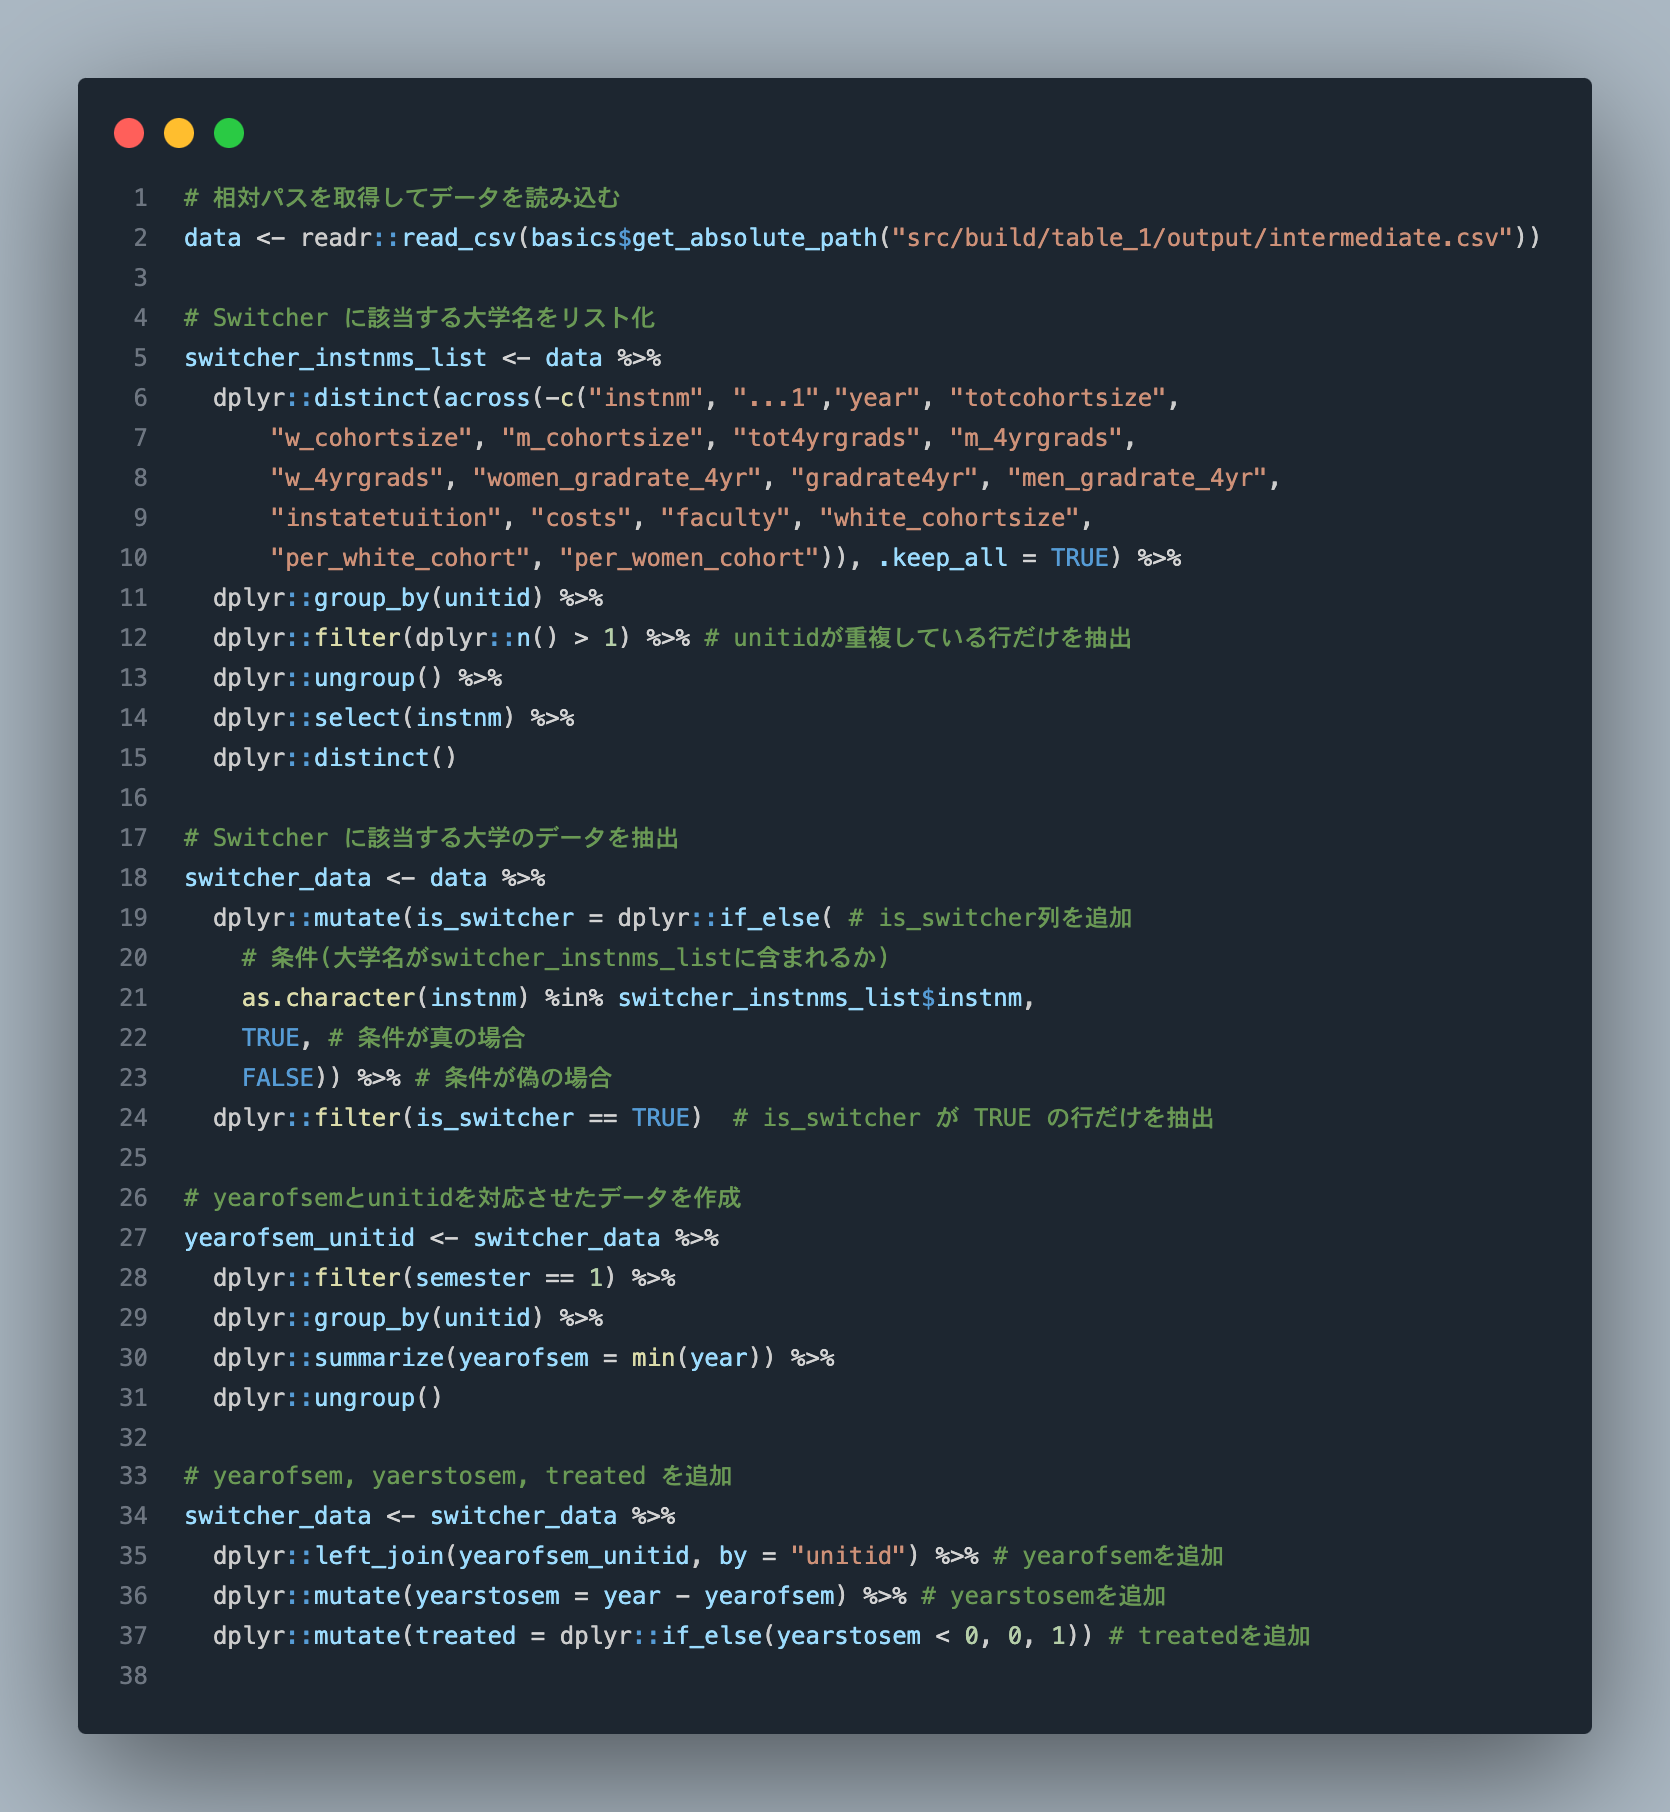
\includegraphics[width = \hsize]{\$HOME/code_box/learn/R/replication-project/src/analyze/output/code.png}

\end{figure}

\subsection*{b-2, 以下の式を推定し、結果について議論しなさい}

s は大学, k は相対年数(yearstosem)

\begin{displaymath}
  \text{Y}_{sk} = \beta_0 + \beta_1 \text{treated}_{sk}  + \epsilon_{sk}
\end{displaymath}


\begin{figure}[H]
  \centering
  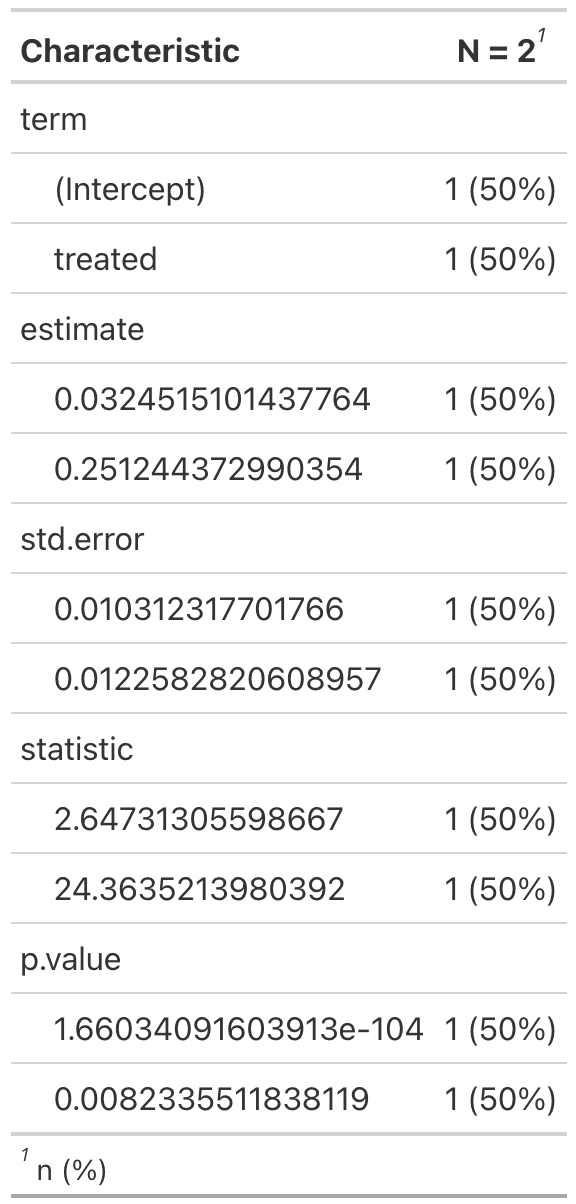
\includegraphics[width = 0.5\hsize]{\$HOME/code_box/learn/R/replication-project/src/analyze/output/figure/lm_result_table.png}

\end{figure}

\begin{figure}[H]
  \centering
  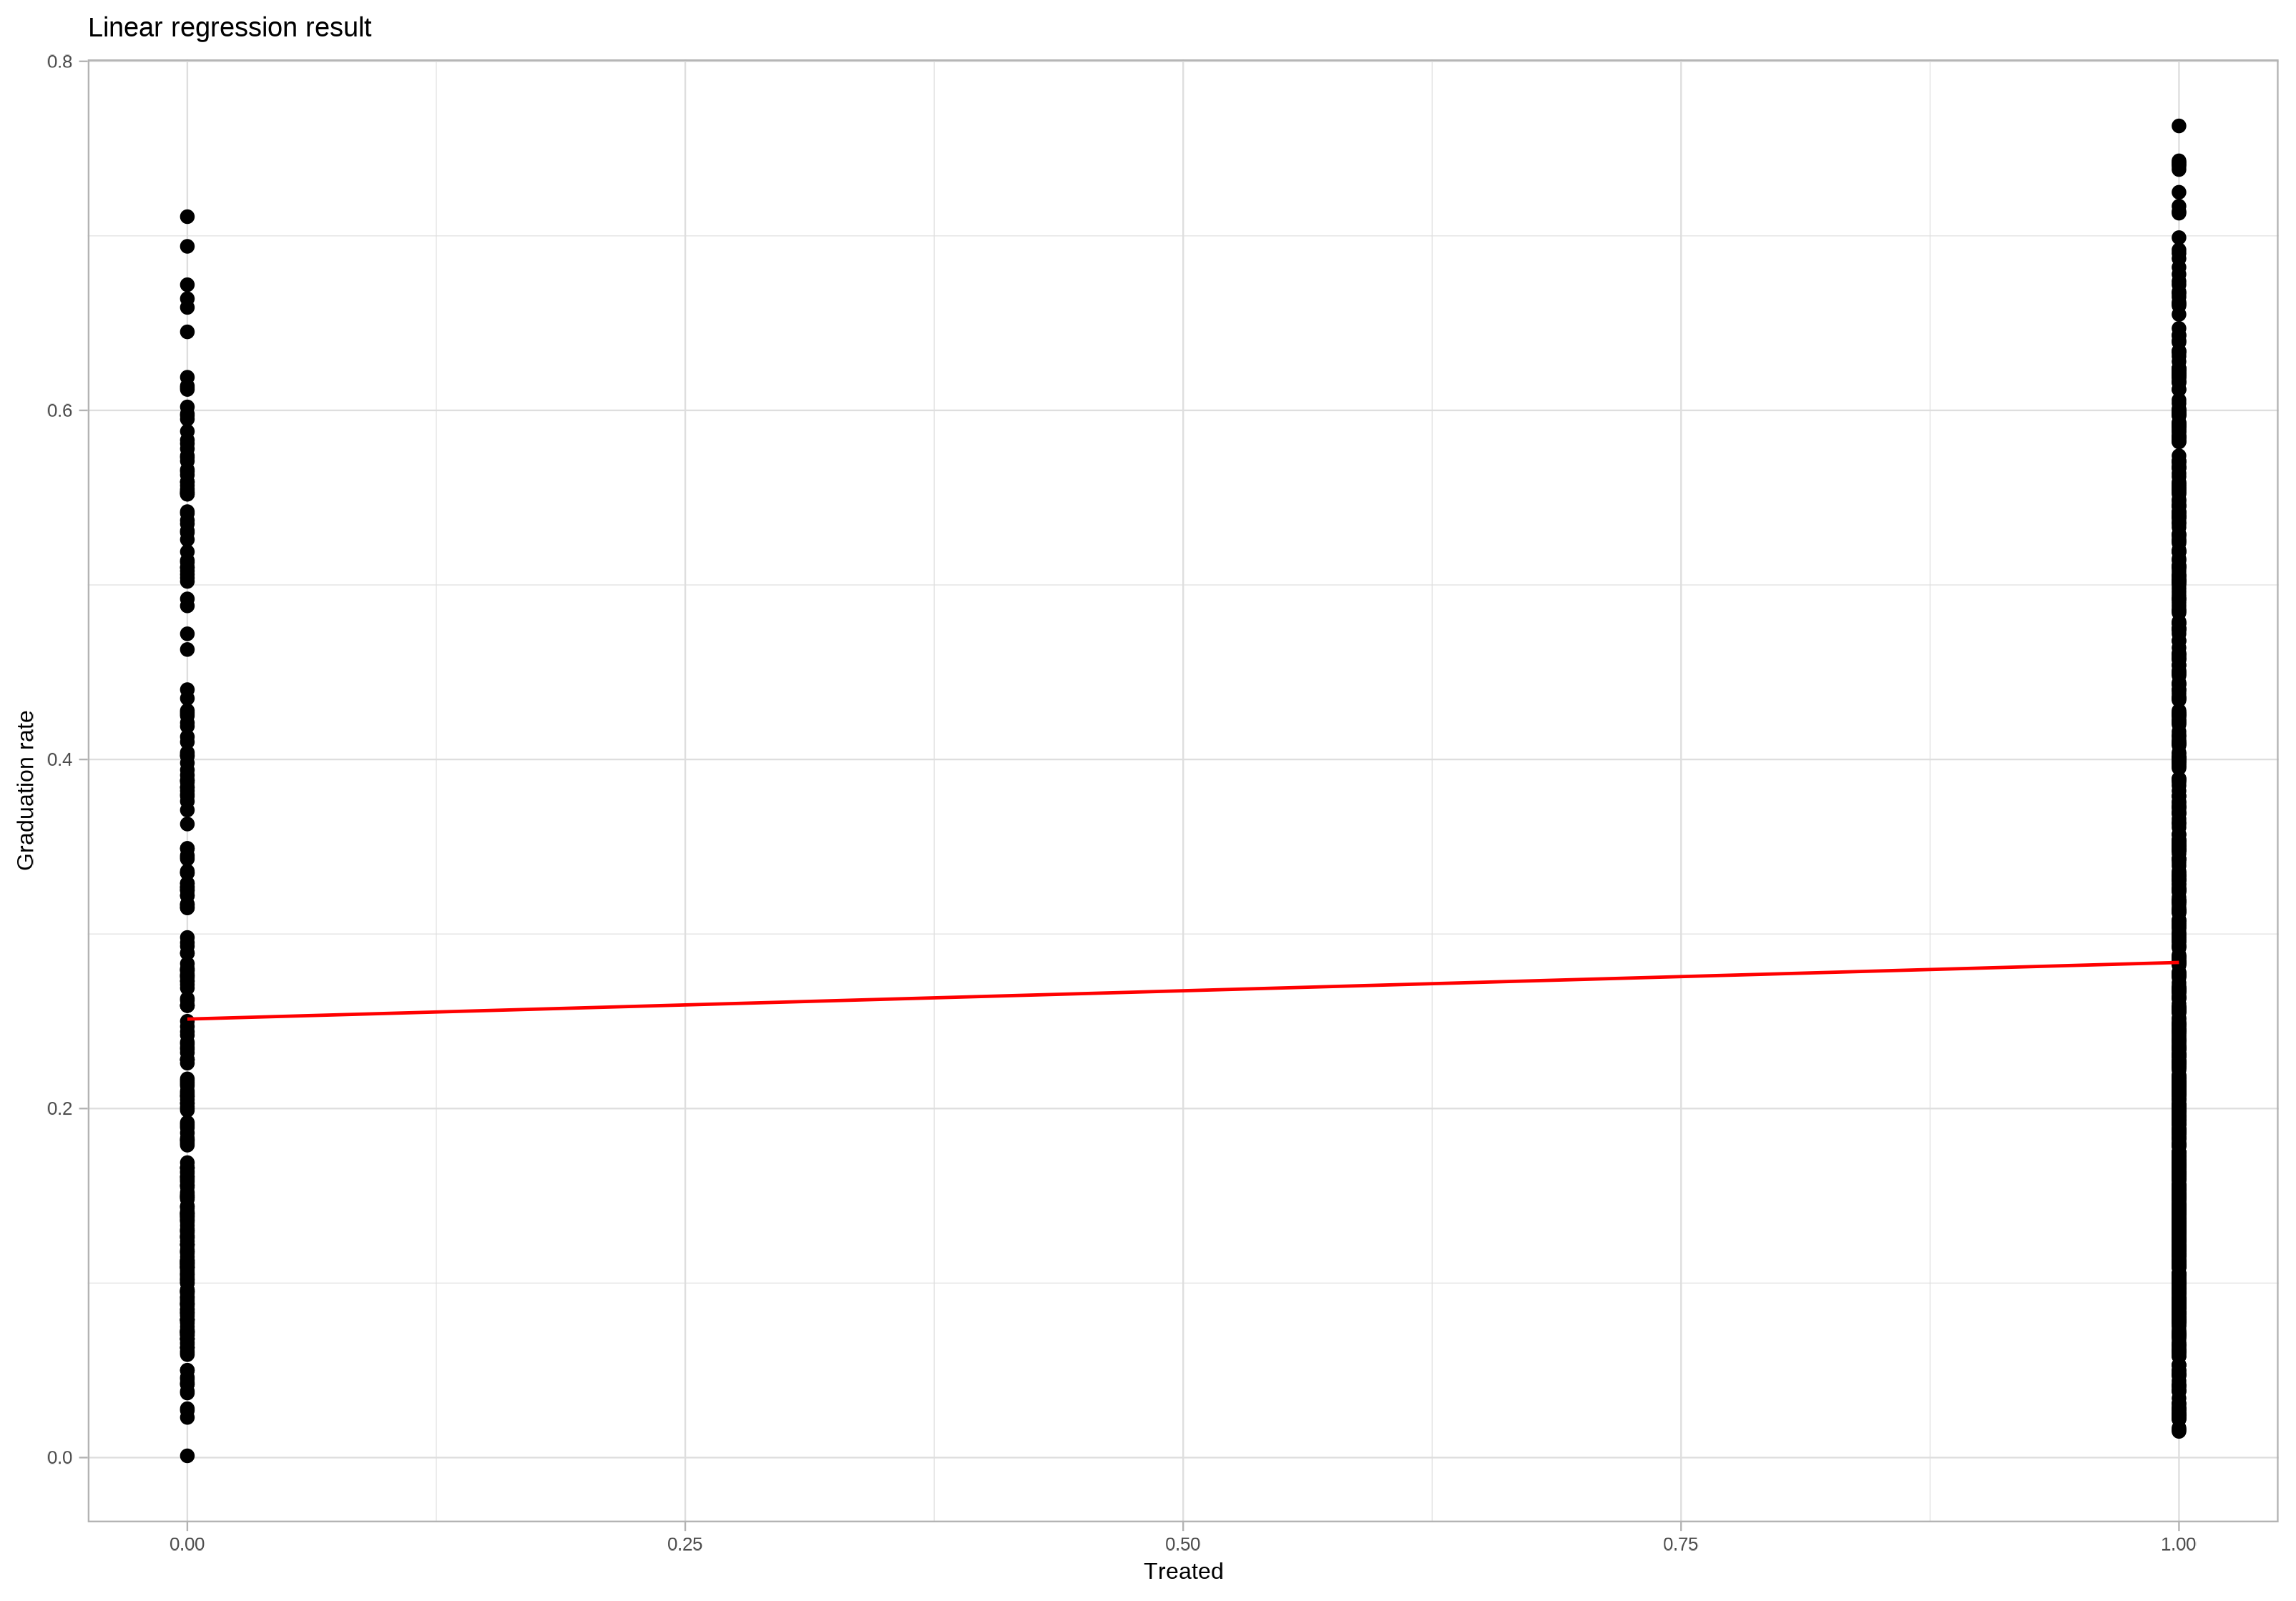
\includegraphics[width = \hsize]{\$HOME/code_box/learn/R/replication-project/src/analyze/output/figure/lm_result_plot.png}

\end{figure}

上記の結果から以下のような回帰式が得られた。

\begin{displaymath}
  \text{Y}_{sk} = 0.2512 + 0.0325 \text{treated}_{sk}  + \epsilon_{sk}
\end{displaymath}

したがって、セメスター制に移行すると、4年卒業率が 3.25\%(SD 1.23\%) 上昇するという結果が得られた。

\subsection*{b-3, 数式の問題点を指摘しなさい}

まず、説明変数が一つと少ないため、その他の変数が目的変数へ与える効果を考慮できていない。さらに、treatedがダミー変数であるためセメスター制へ移行した後の効果の推移を考慮できていない。



\end{document}
